\begin{figure}[ht]
    \centering
    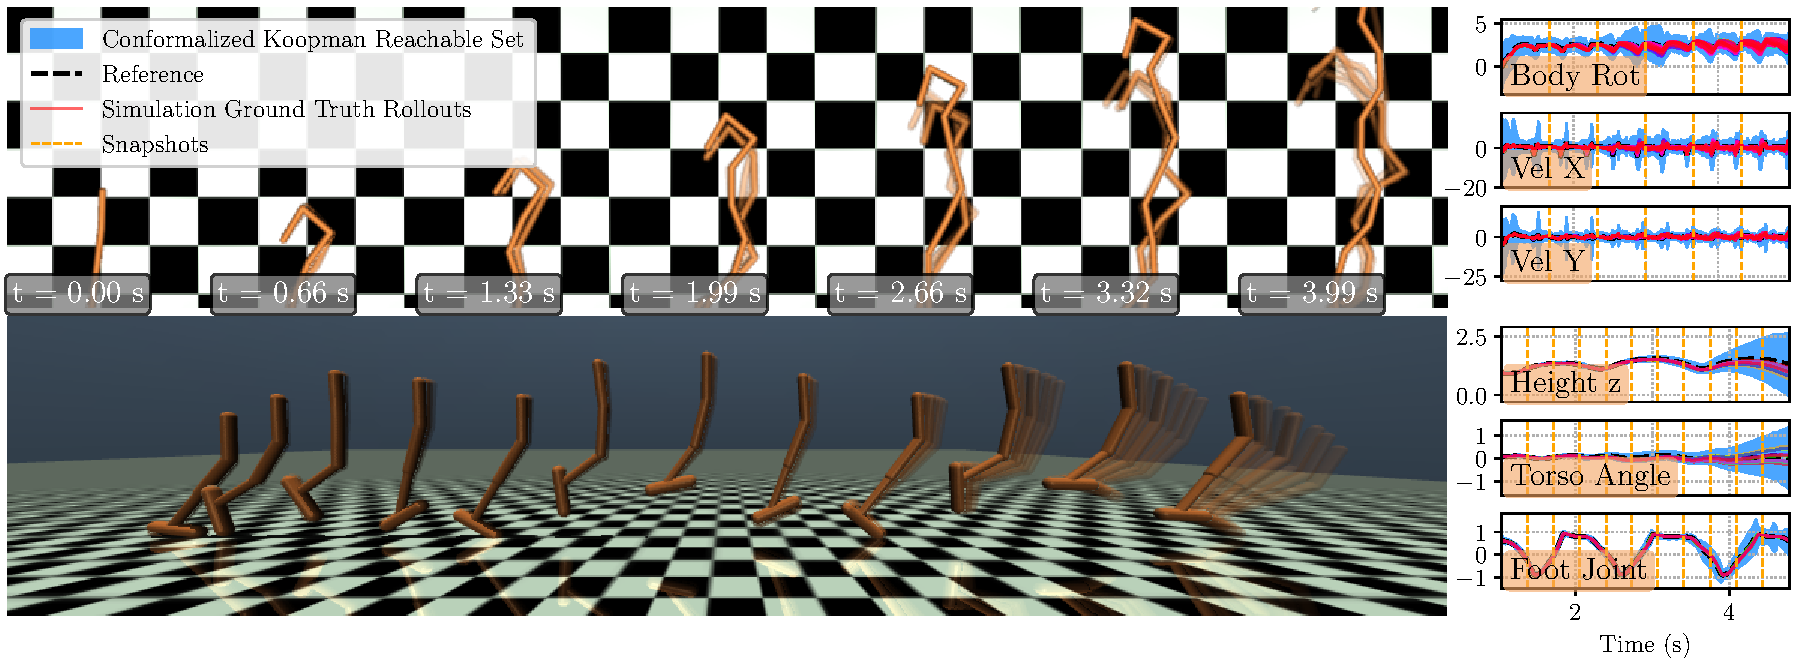
\includegraphics[width=\linewidth]{img/frontfig/Combined_Front_Fig.pdf}
    \caption{Executed trajectories / reachable sets for a 28D MuJoCo swimmer (a); 11D hopper (b).}
    \vspace{-12pt}
    \label{fig:hopper}
\end{figure}

\section{Introduction}
\label{introduction}

Computing reachable sets, i.e., the set of states reachable over a time horizon, is key to robot safety. However, reachability analysis for robots is difficult as they often (i) lack analytical models, (ii) have high-dimensional nonlinear dynamics, and (iii) require reasoning over long horizons. Even if analytical dynamics are available, challenges (ii) and (iii) cause nonlinear reachability tools \citep{bansal2017HJReach, DBLP:conf/cpsweek/Althoff15} to become prohibitive or to suffer from excessive overapproximation over long horizons \citep{Rober2024CARV}. Data-driven reachability \citep{10772635datadrivenreach, DBLP:journals/fmsd/BakBHKLP25} can be used without analytical models, but can be data-inefficient or lack guarantees that the estimated sets contain all possible trajectories. 
In contrast, linear reachability scales to long horizons and high dimensions \citep{10.1145/3302504.3311792}. The Koopman framework learns linear dynamics in a lifted state space, e.g., via neural networks (NNs), to approximate the nonlinear system \citep{koop_survey}. While computing reachable sets for the Koopman linearization can be more scalable than using the original nonlinear dynamics, existing methods only provide guarantees for the approximate lifted dynamics. Thus, \textit{safety may not hold for the true system} \citep{DBLP:conf/adhs/BakBDGP21, DBLP:journals/fmsd/BakBHKLP25}. Moreover, existing Koopman reachability methods analyze a \textit{single} dynamical system. However, robots often require multiple controllers to complete different tasks, which forces existing methods to recompute reachable sets from scratch for each new controller, which is inefficient. Reusing previously computed information would enable more efficient reachability analysis across controllers.

\looseness-1
To close these gaps in scalability, speed, and reusability, we propose \textbf{ScaRe-Kro} (\underline{Sca}lable \underline{Re}achability via \underline{K}oopman Ope\underline{r}at\underline{o}rs), which uses Koopman theory with an NN lifting function to perform reachability analysis and control. Unlike prior Koopman reachability methods for autonomous systems, we also design a linear controller in this lifted space to track a distribution of reference trajectories, each completing a different task. ScaRe-Kro efficiently computes closed-loop reachable sets under the induced \textit{linear tracking error dynamics} in the lifted Koopman space and maps them to the original state space via NN verification tools. To account for Koopman model error, we apply conformal prediction (CP) to derive statistically-valid error bounds. By inflating the mapped reachable sets with these CP bounds, they are guaranteed to contain the \textit{true system trajectories} with a user-specified probability (e.g., 97.5\%). Moreover, as the CP bounds are calibrated across the trajectory distribution, they can be reused across different references and thus closed-loop systems, unlike prior Koopman approaches that certify only a single autonomous system. Overall, using linear reachability and CP, our method enables scalable data-driven probabilistic verification and control, improving both efficiency and conservativeness over prior work. Our contributions are:

\begin{enumerate}
  \setlength{\itemsep}{0pt}
  \setlength{\parskip}{0pt}
  \setlength{\parsep}{0pt}
  \setlength{\topsep}{0pt}
  \setlength{\partopsep}{0pt}
  \item A scalable Koopman-based reachability framework for unknown nonlinear dynamics, using NN lifting functions and NN verification to estimate reachable sets in the original state space.
  \item An approach for inflating the resulting Koopman reachable sets using CP, to obtain probabilistic guarantees of overapproximation for the \textit{true} dynamics.
  \item Control design in the lifted space for closed-loop tracking of a reference trajectory distribution, with CP-based inflation bounds calibrated to be reusable across the distribution.
  \item Extensive evaluation, showing reliable verification for high-dimensional robotic systems (up to 28D), outperforming baselines in safety rate, computation speed, and conservativeness.
\end{enumerate}
